\section{Data}
\label{sec:data}
Luminous red galaxies are massive galaxies that lack active star formation and considered as one of the highly biased tracers of large scale structure. They are widely targeted in previous galaxy surveys \mr{CITE}, and their clustering and redshift properties are well known \mr{CITE}. We use the photometric DESI Luminous Red Galaxies (LRG), selected from the imaging surveys \citep{dey2018overview} using color-magnitude cuts described in the $g$, $r$, $z$, and $W1$ bands \citep[see,][]{zhou2021clustering}, and summarized in Tab. \ref{tab:ts}. The LRG sample are masked for bright stars, foreground bright galaxies as well as clusters of galaxies\footnote{See \url{https://www.legacysurvey.org/dr9/bitmasks/}}, and then binned into \textsc{HEALPix} \citep{gorski2005healpix} at $\textsc{nside}=256$ to construct the LRG density field, with an average density of $800$ deg$^{-2}$ with a coverage around $14000$ square degrees of the sky. Fig. \ref{fig:ng} shows observed density field of DR9 LRGs in deg$^{-2}$. There are some disconnected islands, hereafter referred to as \textit{spurious islands}, in the DECaLS North region at Declination below $-11$, which are removed from the sample to minimize potential calibration issues. Additionally, parts of the DECaLS South with Declination below $-30$ are cut from the sample, since similar calibration issues might infect our analysis. Section \ref{sec:results} presents how these cuts might alter constraints. DESI imaging is a multi-epoch dataset, and thus LRG density map is accounted for pixel incompleteness using a catalog of random points, uniformly scattered over the footprint with the same cuts and masks as DR9 LRGs. Fig. \ref{fig:nz} shows the redshift distribution of DR9 LRGs inferred from DESI Survey Validation \mr{CITE} and the evolution of  galaxy bias for our LRG sample adapted from \cite{zhou2021clustering}, consistent with the assumption of constant clustering amplitude. 

\begin{table*}
  \begin{center}
    \caption{Selection criteria for the LRG targets.}
    \label{tab:ts}
    \begin{tabular}{lc}
    \hline
      \textbf{Criterion} &\textbf{Description}\\
      \hline   
     \textbf{DECaLS} & \\ 
     $z_{\rm fiber} < 21.7$  & faint limit  \\
     $z - W1 > 0.8 \times (r - z) - 0.6$ & Stellar rejection  \\
     $[(g-r >1.3)~{\rm AND}~((g-r) > -1.55*(r-W1) + 3.13)]~{\rm OR}~(r -W 1 > 1.8)$ & Remove low-z galaxies \\
     $[(r-W1 > (W1 - 17.26)*1.8)~{\rm AND}~(r - W1 > W1 - 16.36)]~{\rm OR}~(r-W1 > 3.29)$ & Luminosity cut \\ 
    \hline
     \textbf{BASS+MzLS} & \\ 
     $z_{\rm fiber} < 21.71$  & faint limit  \\
     $z - W1 > 0.8 \times (r - z) - 0.6$ & Stellar rejection  \\
     $[(g-r >1.34)~{\rm AND}~((g-r) > -1.55*(r-W1) + 3.23)]~{\rm OR}~(r -W 1 > 1.8)$ & Remove low-z galaxies \\
     $[(r-W1 > (W1 - 17.24)*1.83)~{\rm AND}~(r - W1 > W1 - 16.33)]~{\rm OR}~(r-W1 > 3.39)$ & Luminosity cut \\ 
      \hline
      \end{tabular}
  \end{center}
\end{table*}


\begin{figure}
    \centering
    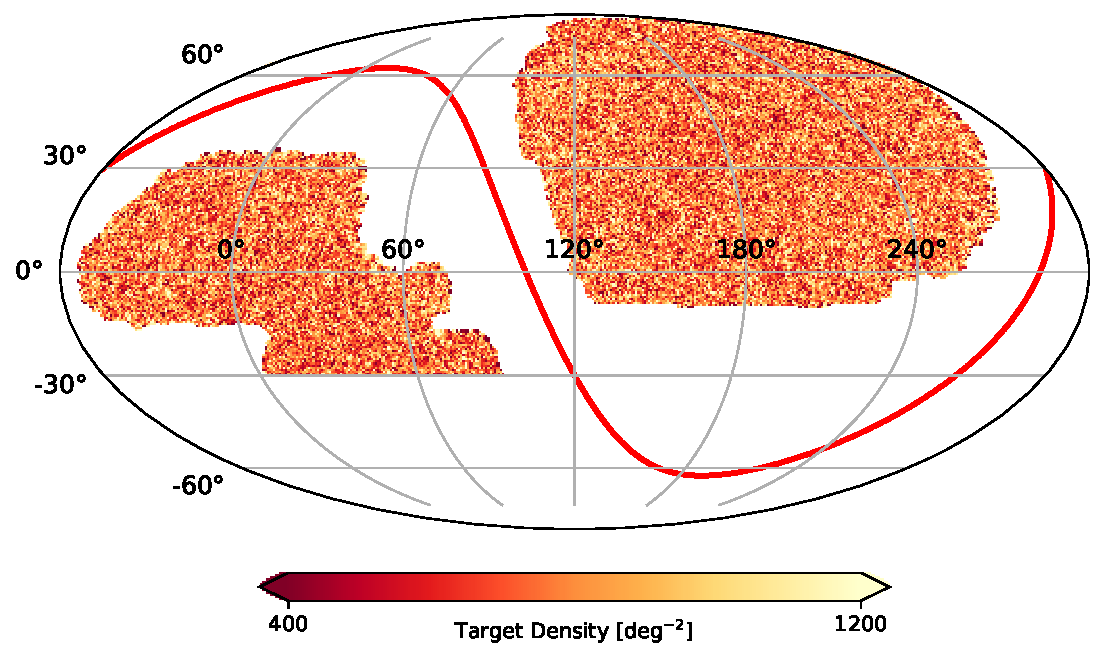
\includegraphics[width=0.45\textwidth]{figures/lrgdens.pdf}
    \caption{Observed density field of DESI Luminous Red Galaxies Data Release 9 in deg$^{-2}$. Spurious islands from the DECaLS North footprint at Declination below $-11$ and parts of the DECaLS South with Declination below $-30$ are dropped from the DR9 sample due to potential calibration issues.}
    \label{fig:ng}
\end{figure}


\begin{figure}
    \centering
    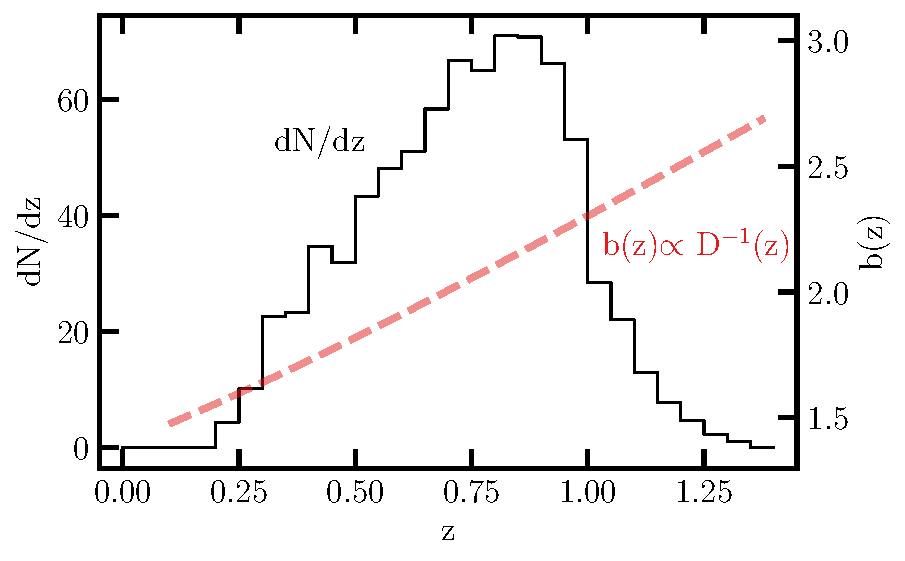
\includegraphics[width=0.45\textwidth]{figures/nz_lrg.pdf}
    \caption{Redshift distribution and bias evolution of DESI LRGs with the assumption of constant clustering amplitude.}
    \label{fig:nz}
\end{figure}


We study the correlation coefficient between the LRG density map and potential sources of systematic error, mapped into \textsc{HEALPix} at the same \textsc{nside}. The maps used in this work are local stellar density constructed from point-like sources with a g-band magnitude in the range $12 \leq g < 17$ from Gaia Data Release 2 \citep[see,][]{gaiadr2, myers2022},  Galactic extinction E[B-V] from \cite{schlegel1998maps}, and other imaging properties including survey depth (galaxy depth in grz and PSF depth in W1) and seeing in grz from DESI imaging. Fig. \ref{fig:pcc} shows the Spearman correlation between galaxy density and imaging properties.

\begin{figure}
    \centering
    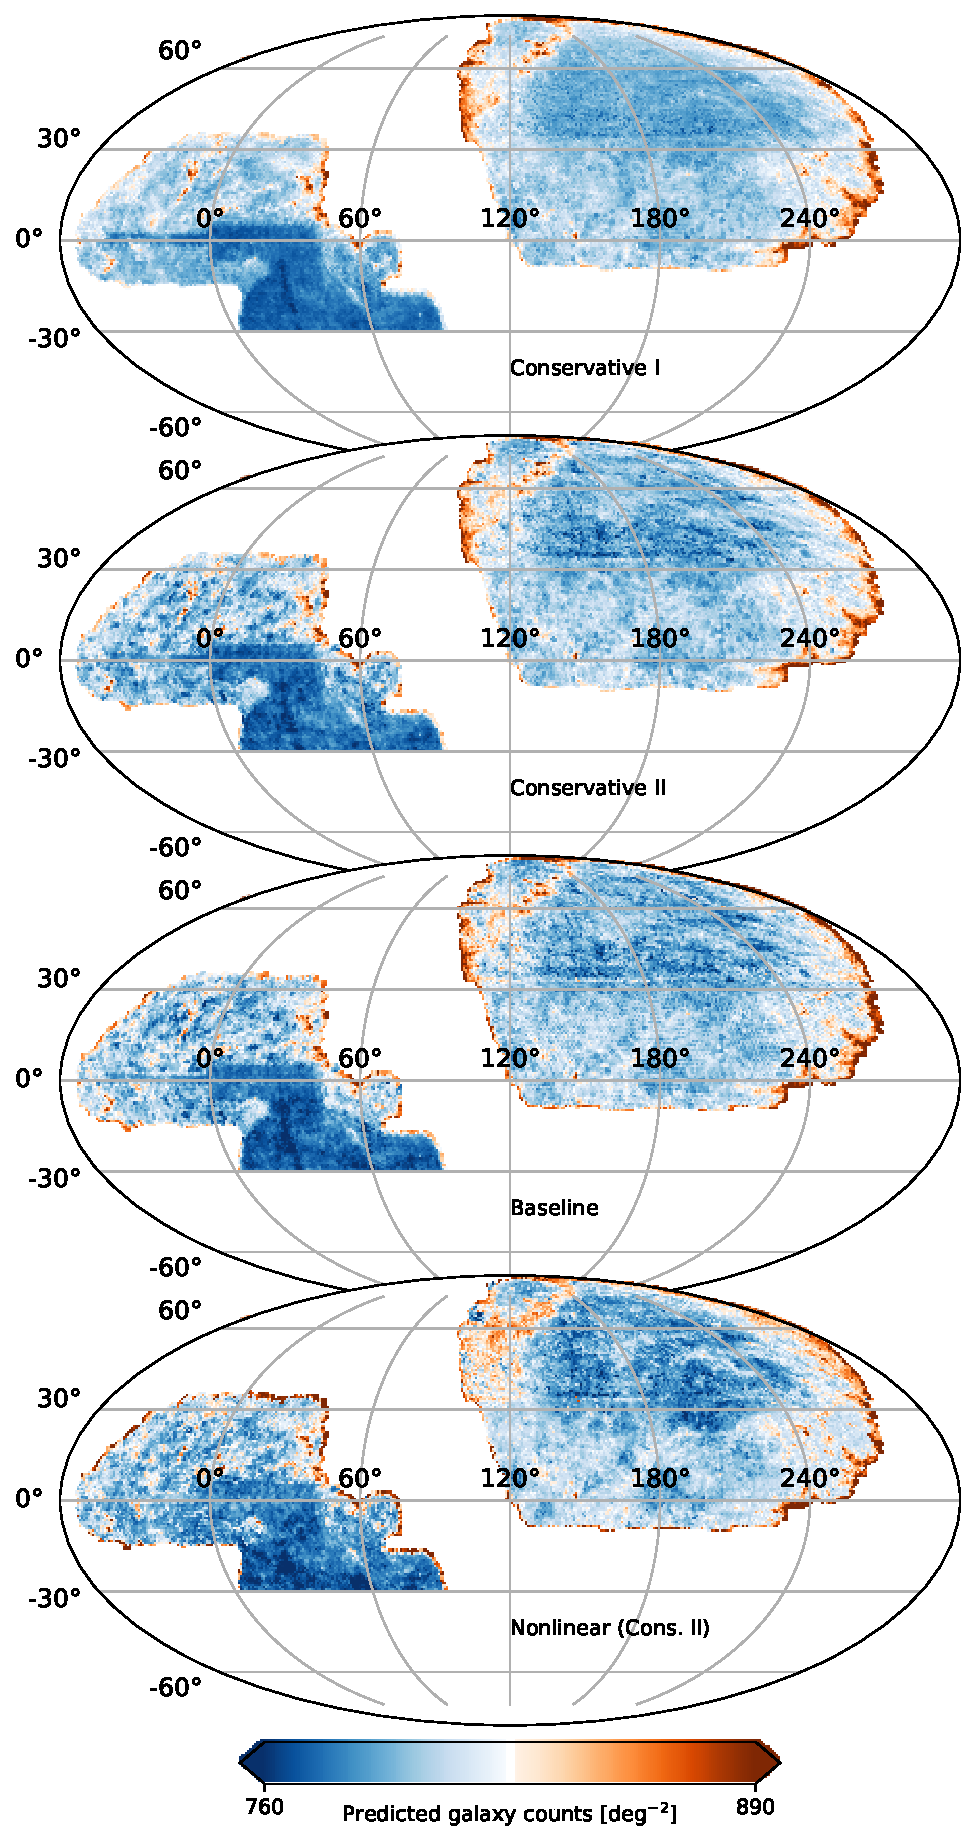
\includegraphics[width=0.45\textwidth]{figures/npred.pdf}
    \caption{Predicted galaxy counts from template regression. Baseline approach uses imaging maps from Zhou et al. (2022): EBV, galaxy depth in rgz, psfdepth in W1, and psfsize in grz. Conservative I uses EBV and galaxy depth in z, and Conservative II uses EBV, galaxy depth in z, and psfsize in r. In all approaches, the models are regressed on BASS+MzLS, DECaLS North, and DECaLS South separately.}
    \label{fig:npred}
\end{figure}

\begin{figure}
    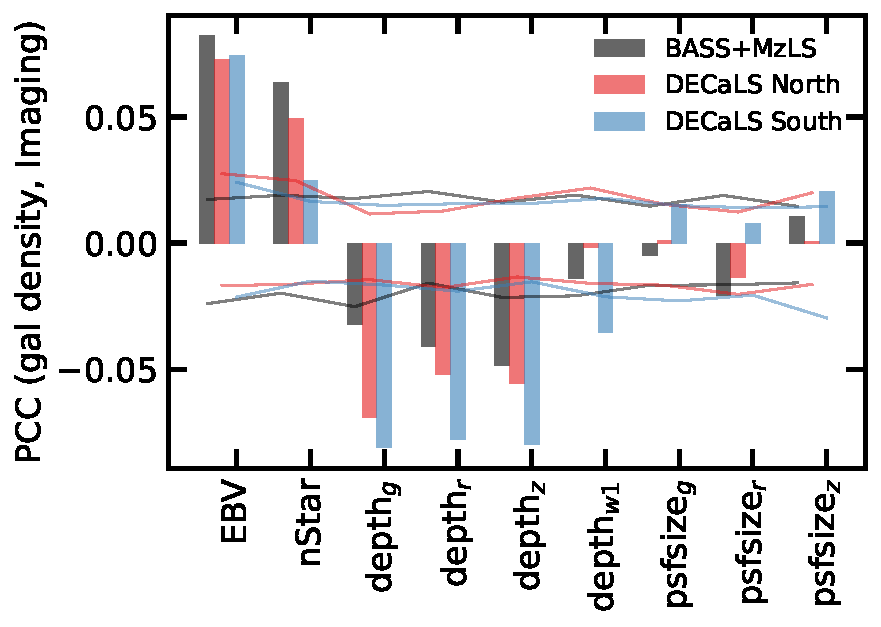
\includegraphics[width=0.45\textwidth]{figures/pcc.pdf} 
    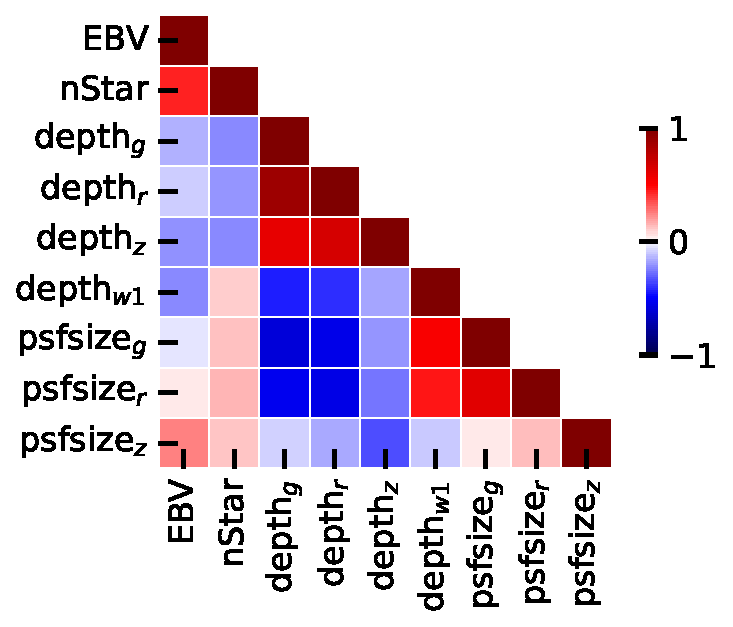
\includegraphics[width=0.45\textwidth]{figures/pccx.pdf}     
    \caption{Top: Pearson-r correlation coefficient between galaxy density and imaging properties in the three imaging regions (top) and between imaging properties themselves for the full DESI footprint (bottom). Solid curves represent the range of correlations observed in 100 randomly selected mock realizations.}
    \label{fig:pcc}
\end{figure}
